\documentclass[a4paper, 12pt]{article}		% general format

%%%% Charset
\usepackage{cmap}							% make PDF files searchable and copyable
\usepackage[utf8]{inputenc}					% accept different input encodings
\usepackage[T2A]{fontenc}					% russian font
\usepackage[russian]{babel}					% multilingual support (T2A)

%%%% Graphics
\usepackage[dvipsnames]{xcolor}			% driver-independent color extensions
\usepackage{graphicx}						% enhanced support for graphics
\usepackage{wrapfig}						% produces figures which text can flow around

%%%% Math
\usepackage{amsmath}						% American Mathematical Society (AMS) math facilities
\usepackage{amsfonts}						% fonts from the AMS
\usepackage{amssymb}						% additional math symbols

%%%% Typograpy (don't forget about cm-super)
\usepackage{microtype}						% subliminal refinements towards typographical perfection
\linespread{1.3}							% line spacing
\usepackage[left=2.5cm, right=1.5cm, top=2.5cm, bottom=2.5cm]{geometry}
\setlength{\parindent}{0pt}					% we don't want any paragraph indentation

%%%% Other
\usepackage{url}							% verbatim with URL-sensitive line breaks
\usepackage{listings}						% typeset source code listings
\lstset{
	breaklines=true, % Перенос длинных строк
	basicstyle=\ttfamily\footnotesize, % Шрифт для отображения кода
	frame=tblr % draw a frame at all sides of the code block
	tabsize=2, % tab space width
	showstringspaces=false, % don't mark spaces in strings
	% Настройка отображения номеров строк
	numbers=left, % Слева отображаются номера строк
	stepnumber=1, % Каждую строку нумеровать
	numbersep=5pt, % Отступ от кода
}
\renewcommand{\lstlistingname}{Листинг} % Переименование Listings в нужное именование структуры
%------------------------------------------------------------------------------
\author{Семён Мартынов\\<semen.martynov@gmail.com>}
\title{Отчет по лабораторной работе 1:\\\LaTeX{} Git GPG}
\begin{document}
\maketitle
\tableofcontents{}

%------------------------------------------------------------------------------
\newpage
\section{Cистема верстки \TeX{} и расширения \LaTeX{}}

\subsection{Цель работы}

Изучение принципов верстки \TeX{}, создание первого отчёта.

\subsection{Ход работы}

Файл .tex представляет из себя обычный текстовый файл содержащий макрокоманды текстовой разметки.

\subsubsection{Компиляция в командной строке}

\begin{itemize}
	\item{ latex генерирует файл в формате DVI (\textbf{D}e\textbf{V}ice \textbf{I}ndependent — аппаратно независимый) не предназначенный для чтения человеком, но содержит двоичные данные, описывающие визуальное представление документа способом, не ориентированным на какой-либо формат изображения, монитор или принтер.  Файлы DVI обычно подаются на вход другой программы (называемой DVI-драйвером), которая преобразует их в графические данные.
	\begin{verbatim}latex report.tex
	\end{verbatim}}
	
	\item {xdvi одна из программ DVI-драйверов, позволяющих отображать данные в формате DVI в X Window системах
	\begin{verbatim}xdvi report.dvi
	\end{verbatim}
	
	Результат показан на рисунке 1.
	
	\begin{figure}[h!]
	\centering
	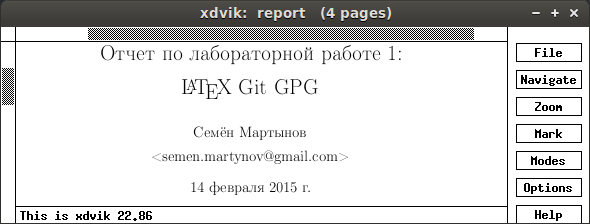
\includegraphics[scale=0.83]{res/xdvi}
	\caption{Запуск xdvi}
	\end{figure}
	}
	
	\item {pdflatex позволяет сразу сгенерировать pdf файл. Главное различие между TeX и pdfLaTeX состоит в том, что TeX после трансляции выдаёт DVI-файлы, а pdfTeX -- PDF-файлы, минуя цепочку преобразований DVI -> PS -> PDF.
	\begin{verbatim}pdflatex report.tex
	\end{verbatim}}

\end{itemize}

\subsubsection{Оболочка TexMaker}

Texmaker является мощным редактором текста и исходного кода, работающий с языком разметки LaTeX. Он позволяет форматировать текст и готовить многостраничные документы к печати. Редактор предоставляет возможность работы с библиографическими списками, оглавлением и другими атрибутами профессионального оформления. В Texmaker есть так же возможность конвертирования документов в различные форматы, функции сворачивания блоков кода и автозавершения кода, встроенный просмотрщик PDF документов и многое другое. Внешний вид редактора представлен на рисунке 2.

\begin{figure}[h!]
\centering
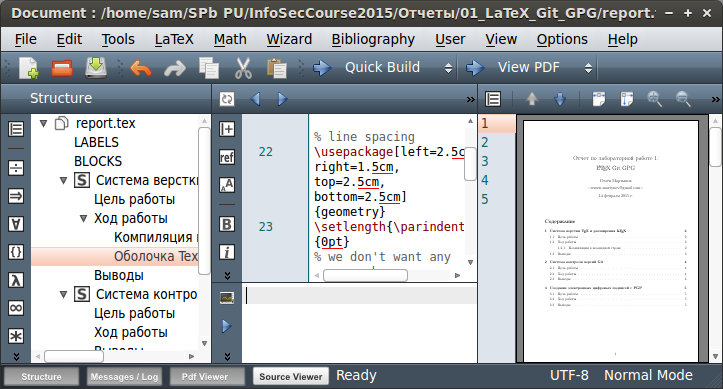
\includegraphics[scale=0.65]{res/TexMaker}
\caption{Редактор TexMaker}
\end{figure}

Texmaker обладает двумя интересными возможностями: быстрый старт и быстрая сборка.

Быстрый старт (рисунок 2) позволяет задать преамбулу (главные особенности - класс, размер бумаги, кодировку...) документа. Имеется возможность создать собственную модель преамбулы в редакторе.

\begin{figure}[h!]
\centering
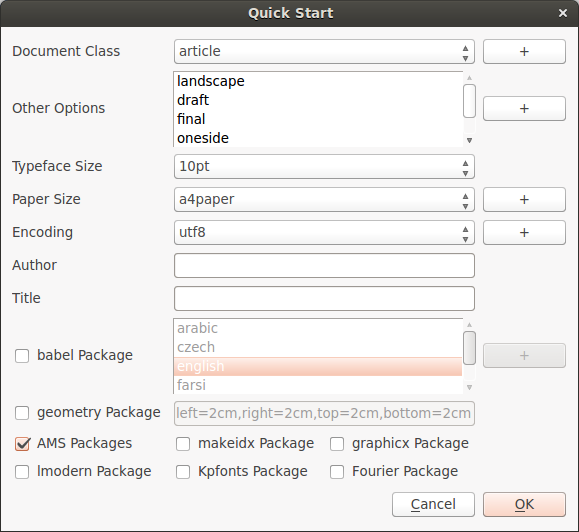
\includegraphics[scale=0.65]{res/QuickStart}
\caption{Редактор TexMaker}
\end{figure}

Самый простой способ скомпилировать документ это использовать команду "Быстрая сборка". Задать последовательность команд используемых быстрой сборкой можно в диалоге "Настроить Texmaker". Если в коде документа содержатся ошибки, Texmaker напишет об этом в окне сообщений.

\subsubsection{Классы документов}

Каждый созданный файл в \LaTeX{} начинается с команды \verb+\documentclass[...]{…}+, в фигурных скобках которой задаются параметры оформления стиля документа, а в квадратных — список классовых опций.

Всего же в \LaTeX{} 5 основных классов документов: article (для статей), report (для верстки небольших книг, статей, разбитых на главы), book (для верстки книг), proc (возможно использовать для докладов) и letter (для оформления деловых писем). Помимо этих основных, есть ещё множество дополнительных классов, таких как beamer.

\subsubsection{Подключаемые пакеты}

В \LaTeX{} можно применять специфические, отличные от изначальных, настройки (поля, списки и таблицы, библиографические ссылки и прочее). Для этого используются пакеты расширений, подключаемые в "шапке" документа.

Пример:
\begin{verbatim}\usepackage[russian]{babel} % Пакет поддержки русского языка
\end{verbatim}

\subsubsection{Вёрстка формул}

Вёрстка формул не представляет никакой сложности.

Система дифференциальных уравнений Рёсслера

\begin{center}
$\left \{ \begin{matrix} \frac{dx}{dt} = -y - z \\ \frac{dy}{dt} = x + ay \\ \frac{dz}{dt} = b + z(x-c) \end{matrix} \right.  ;$
\end{center}

Массив связных осцилляторов Рёсслера:
\begin{center}
$\dot{x_i} = -\omega_iy_i - z_i +k(2x_i - x_{i-1} - x_{i+i})$,\\
$\dot{y_i} = \omega_ix_i - ay_i$,\\
$\dot{z_i} = b + z_i(x_i - c)$,
\end{center}


\subsection{Выводы}

\LaTeX{} наиболее популярный набор макрорасширений (или макропакет) системы компьютерной вёрстки \TeX{}, который облегчает набор сложных документов.

Пакет позволяет автоматизировать многие задачи набора текста и подготовки статей, включая набор текста на нескольких языках, нумерацию разделов и формул, перекрёстные ссылки, размещение иллюстраций и таблиц на странице, ведение библиографии и др. Кроме базового набора существует множество пакетов расширения \LaTeX{}.

Термин \LaTeX{} относится только к языку разметки, он не является текстовым редактором. Для того, чтобы создать документ с его помощью, надо набрать .tex-файл с помощью какого-нибудь текстового редактора. В принципе, подойдёт любой редактор, но большая часть людей предпочитает использовать специализированные, которые так или иначе облегчают работу по набору текста \LaTeX{}-разметки.

Будучи распространяемым под лицензией LaTeX Project Public License, \LaTeX{} относится к свободному программному обеспечению.

%------------------------------------------------------------------------------
\newpage
\section{Система контроля версий Git}

\subsection{Цель работы}
Изучить систему контроля версий Git, освоить основные приёмы работы с ней.

\subsection{Ход работы}

\begin{itemize}

\item{Получить содержимое репозитория
\begin{verbatim}git clone git@github.com:SemenMartynov/InfoSecCourse2015.git
\end{verbatim}}

\item{Добавить новую папку и первого файла под контроль версий
\begin{verbatim}cd InfoSecCourse2015/
mkdir tmp
cd tmp
echo 1 >> file
git add --all
\end{verbatim}}

\item{Зафиксировать изменения в локальном репозитории
\begin{verbatim}git commit -a -m "file added"
\end{verbatim}}

\item{Внести изменения в файл и просмотреть различия
\begin{verbatim}echo 2 >> file
git diff master:./file ./file
\end{verbatim}}

\item{Отменить локальные изменения
\begin{verbatim}git reset HEAD ./file
git checkout ./file
\end{verbatim}}

\item{Внести изменения в файл и просмотреть различия
\begin{verbatim}echo 3 >> file
git diff master:./file ./file
\end{verbatim}}

\item{Зафиксировать изменения в локальном репозитории, зафиксировать изменения в центральном репозитории
\begin{verbatim}git commit -a -m "file changed"
git push
\end{verbatim}}

\item{Получить изменения из центрального репозитория
\begin{verbatim}git pull
\end{verbatim}}

\item{Поэкспериментировать с ветками
\begin{verbatim}git branch -v
git checkout -b temp
git checkout master
git merge temp
git branch
git branch -D temp
git branch
\end{verbatim}}

\end{itemize}

\subsection{Выводы}

Git распределённая система управления версиями файлов. Git используется многими продуктами с открытым исходным кодом, такими как ядро Linux, Android, GNU Core Utilities, Mesa, Wine, Chromium и т.д. Программа является свободной и выпущена под лицензией GNU GPL версии 2.

Преимущества и недостатки git по сравнению с централизованными системами управления версиями (такими как, например, Subversion) типичны для любой распределённой системы. Если же сравнивать git с «родственными» ей распределёнными системами, можно отметить, что git изначально идеологически ориентирован на работу с изменениями, а не с файлами, «единицей обработки» для него является набор изменений, или патч. Эта особенность прослеживается как в структуре самой системы (в частности — в структуре репозитория), так и в принципах построения команд; она отражается на производительности системы в различных вариантах её использования и на достоинствах и недостатках git по сравнению с другими DVCS.

%------------------------------------------------------------------------------
\newpage
\section{Cоздание электронных цифровых подписей c PGP}

\subsection{Цель работы}
Научиться создавать сертификаты, шифровать файлы и ставить ЭЦП.

\subsection{Ход работы}

\subsubsection{Знакомство с пакетом Kleopatra}

Kleopatra это графический интерфейс к GnuPG и предназначенных для работы под окружением KDE и портированный на MS Windows (доступные в составе пакета Gpg4win). Внешний вид пакета представлен на рисунке 4.

\begin{figure}[h!]
\centering
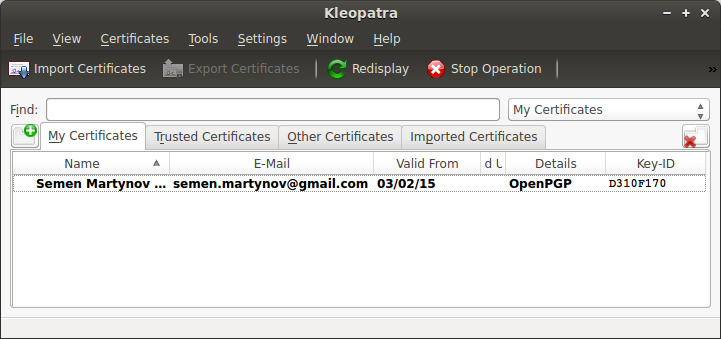
\includegraphics[scale=0.67]{res/Kleopatra}
\caption{Графический интерфейс Kleopatra}
\end{figure}

При помощи мастера, графический интерфейс позволяет создать сертификат. Его текстовый вид представлен в листинге 1.

\lstinputlisting[language={},caption={Сертификат в формате asc (ASCII Armored file)}]{res/502F30EAC9B37E1C9700A07A8A68917DD310F170.asc}

Имея свой сертификат, можно подписать любой имеющийся документ. Цифровая подпись сохраняется в отдельный файл с расширением sig. Если зашифровать файл \textit{rfc7169.txt}, то подпись будет сохранена в файле \textit{rfc7169.txt.sig} (см. рис. 5).

\begin{figure}[h!]
\centering
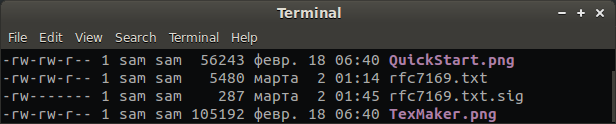
\includegraphics[scale=0.8]{res/rfcsig}
\caption{Файл RFC7169 с подписью}
\end{figure}

Программа позволяет импортировать чужие сертификаты, и проверять подписи. На рисунке 6 показан итог импорта чужого файла.

\begin{figure}[h!]
\centering
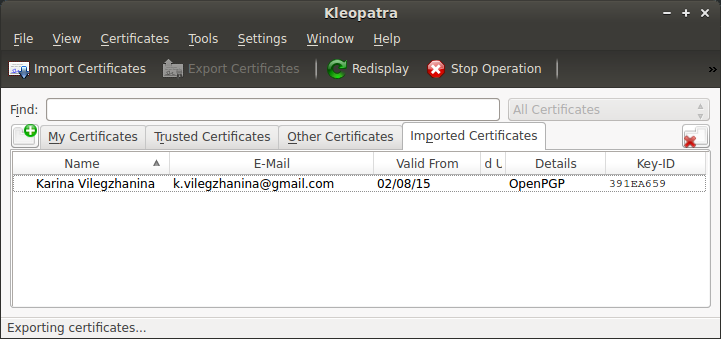
\includegraphics[scale=0.67]{res/Kleopatra2}
\caption{Импорт чужого ключа в Kleopatra}
\end{figure}

Если подтвердить достоверность импортированного ключа, то его можно использовать для проверки чужой подписи. На рисунке 7 показана проверка файла \textit{myfirst.pdf}.

\begin{figure}[h!]
\centering
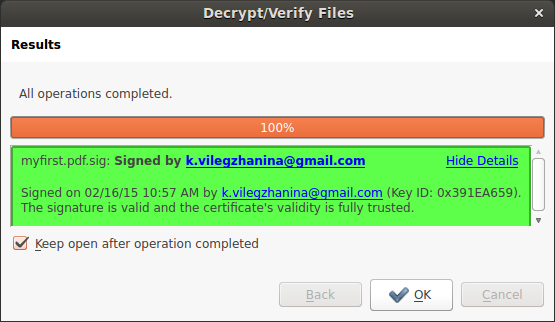
\includegraphics[scale=0.67]{res/myfirst_check}
\caption{Результат проверки файла myfirst.pdf}
\end{figure}

\subsubsection{Использовании gpg через интерфейс командной строки}

Результат, полученный при помощи Kleopatra легко повторить используя терминал. Генерация ключа происходит в диалоговом режиме после ввода команды
\begin{verbatim}gpg --gen-key
\end{verbatim}
В процессе работы, мастер создания ключа запросит следующую информацию:
\begin{itemize}
	\item{Тип ключа (по умолчанию это DSA и ElGamal).}
	\item{Размер ключа (с DSA/ElGamal ключами не использую длину больше чем 2048).}
	\item{"срок годности" ключа.}
	\item{Информацию о пользователе (имя, электронный адрес).}
	\item{Пароль для ключа (если нужен).}
\end{itemize}

В процессе генерации ключа, GnuPG использует энтропию. Для способствования её сбору рекомендуется активно двигать мышкой или запустить mp3 в фоновом режиме.

Просмотреть доступные в системе ключи позволяет команда
\begin{verbatim}gpg --list-keys
\end{verbatim}
Её вывод показан на рисунке 7.

\begin{figure}[h!]
\centering
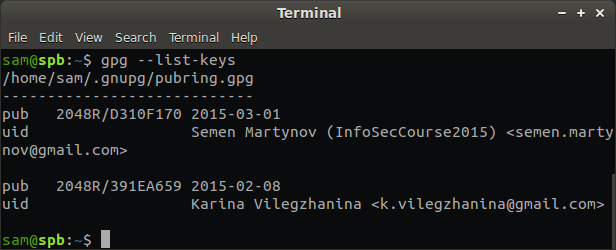
\includegraphics[scale=0.8]{res/gpg-list}
\caption{Список ключей в системе.}
\end{figure}

Для экспорта можно использовать команду (ключ определяется по электронному адресу)
\begin{verbatim}gpg --armor --output john.asc --export john@mail.ru
\end{verbatim}

Для импорта используется
\begin{verbatim}gpg --import tomas.asc
\end{verbatim}

\subsection{Выводы}

Пакет Kleopatra имеет большое количество зависимостей, среди которых akonadi-backend-mysql, akonadi-server, dirmngr, docbook-xml, docbook-xsl, gnupg-agent, gnupg2, gpgsm, icoutils, kate-data, katepart, kde-runtime, kde-runtime-data, kdelibs-bin, kdelibs5-data, kdelibs5-plugins, kdepim-runtime, kdepimlibs-kio-plugins, kdoctools, kleopatra, kubuntu-debug-installer, libaccounts-qt1, libakonadi-calendar4, libakonadi-contact4, libakonadi-kabc4, libakonadi-kcal4, libakonadi-kde4, libakonadi-kmime4, libakonadi-notes4, libakonadi-socialutils4, libakonadiprotocolinternals1, libattica0.4, libbaloocore4, libbaloofiles4, libbaloopim4, libbalooxapian4, libboost-program-options1.54.0, libcalendarsupport4, libdlrestrictions1, libdmtx0a, libepub0, libgpgme++2, libgrantlee-core0, libgrantlee-gui0, libincidenceeditorsng4, libkabc4, libkactivities-bin, libkactivities-models1, libkactivities6, libkalarmcal2, libkatepartinterfaces4, libkcal4, libkcalcore4, libkcalutils4, libkcmutils4, libkde3support4, libkdeclarative5, libkdecore5, libkdepim4, libkdepimdbusinterfaces4, libkdesu5, libkdeui5, libkdewebkit5, libkdgantt2-0, libkdnssd4, libkemoticons4, libkfbapi1, libkfile4, libkgapi2-2, libkholidays4, libkhtml5, libkidletime4, libkimap4, libkio5, libkjsapi4, libkjsembed4, libkldap4, libkleo4, libkmbox4, libkmediaplayer4, libkmime4, libknewstuff3-4, libknotifyconfig4, libkntlm4, libkolab0, libkolabxml1, libkparts4, libkpgp4, libkpimidentities4, libkpimtextedit4, libkpimutils4, libkprintutils4, libkpty4, libkresources4, libkrosscore4, libksba8, libktexteditor4, libktnef4, libkubuntu0, libkxmlrpcclient4, libmailcommon4, libmailimporter4, libmailtransport4, libmessagecomposer4, libmessagecore4, libmessageviewer4, libmicroblog4, libmysqlclient18, libnepomuk4, libnepomukcleaner4, libnepomukcore4abi1, libnepomukquery4a, libnepomukutils4, libntrack-qt4-1, libntrack0, libphonon4, libpimcommon4, libplasma3, libpolkit-qt-1-1, libprison0, libpth20, libqapt2, libqapt2-runtime, libqca2, libqgpgme1, libqjson0, libqmobipocket1, libqrencode3, libqt4-qt3support, libqt4-sql-mysql, libsendlater4, libsignon-qt1, libsolid4, libsoprano4, libstreamanalyzer0, libstreams0, libtemplateparser4, libthreadweaver4, libvirtodbc0, libxerces-c3.1, libxml2-utils, libzip2, mysql-client-core-5.5, mysql-server-core-5.5, nepomuk-core-data, nepomuk-core-runtime, ntrack-module-libnl-0, odbcinst, odbcinst1debian2, oxygen-icon-theme, phonon, phonon-backend-gstreamer, phonon-backend-gstreamer-common, phonon-backend-gstreamer1.0, pinentry-gtk2, pinentry-qt4, plasma-scriptengine-javascript, qapt-batch, scdaemon, sgml-data, shared-desktop-ontologies, soprano-daemon, ttf-dejavu-core, virtuoso-minimal, virtuoso-opensource-6.1-bin, virtuoso-opensource-6.1-common. В общей сложности, эти пакеты требуют порядка 300 мегабайт, что делает использование интерфейса командной строки более предпочтительным вариантом.

\end{document}